\documentclass{beamer}

\usetheme{Madrid}

\usepackage{graphicx}
\usepackage{amsmath}

\title[Necessary Conditions of Political Unification]{External Threats, Linguistic Homogeneity, and Political Unification}
\author{Chen Zeng}
\institute[]{Department of Political Science \\ Renmin University of China}

\begin{document}
	\maketitle
	\begin{frame}{Introduction}
		\begin{columns}
			\begin{column}{.4\textwidth}
				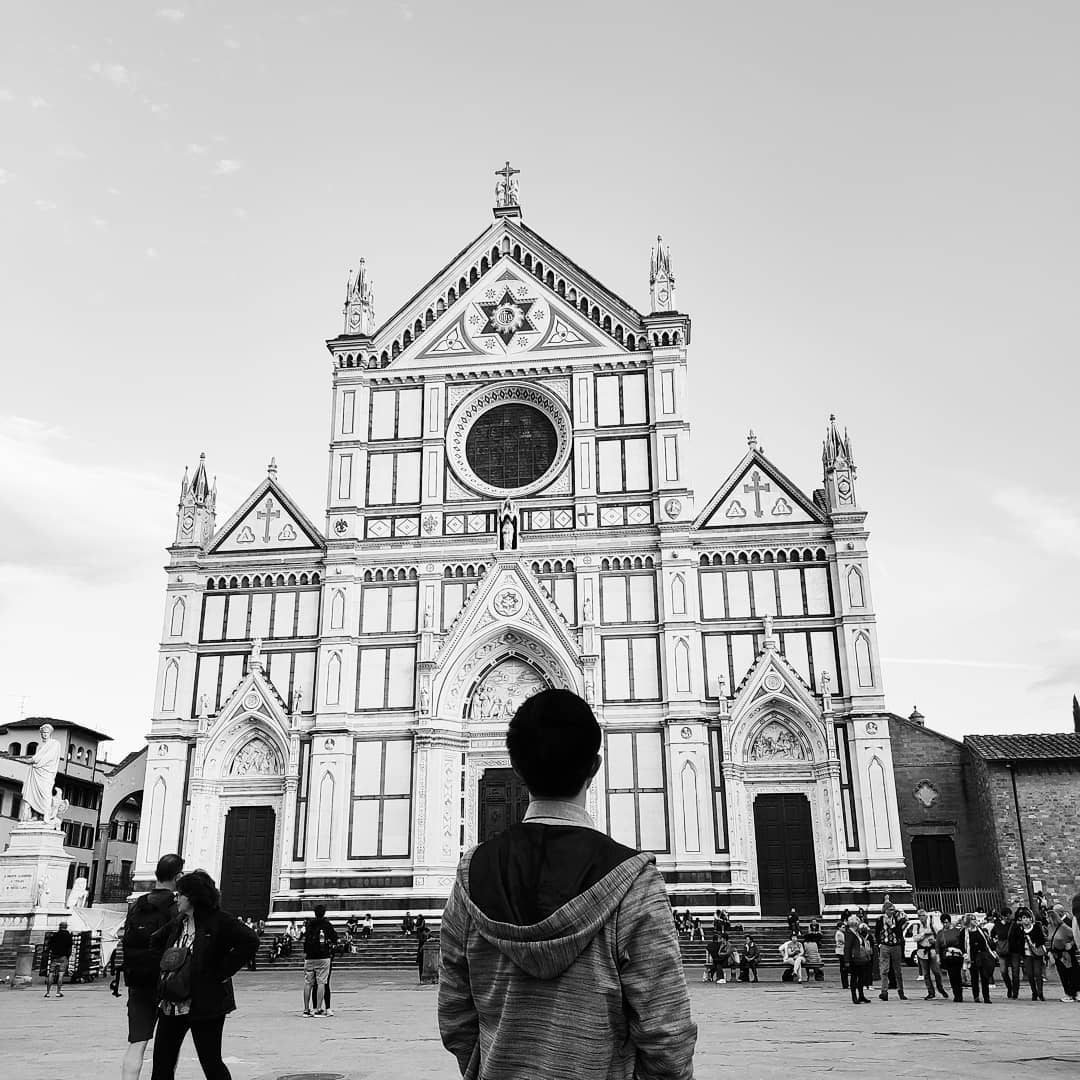
\includegraphics[width=\textwidth]{santa_croce.jpg}
			\end{column}
			\begin{column}{.6\textwidth}
				Niccolò Machiavelli, a Florentine in the 16th century, argued for the unification of Italy, which didn't happen until the \textit{Risorgimento} in 19th century, citing the following reasons:
				\begin{itemize}
					\item Florentine lifestyle
					\item The Italian language, i.e. Tuscan dialect
					\item Women, god, and heroes
					\item External interference
				\end{itemize}
				Today we look at two key elements in the political unification of states --- external security threats and linguistic homogeneity.
			\end{column}
		\end{columns}
	\end{frame}
	\begin{frame}{Contents}
		\tableofcontents
	\end{frame}
	\section{Conceptualization and Operationalization}
	\subsection{Political Unification}
	\begin{frame}{Political Unification}
		\begin{block}{Definition}
			\begin{description}
				\item[Political unification] occurs when two or more sovereign states merge into one.
			\end{description}
		\end{block}
		\begin{itemize}
			\item Political unification has been one of the most debated areas in the study of political science.
			\item Notable instances included the US (American Revolutionary War), Germany (\textit{Sonderweg}), and Italy (\textit{Risorgimento}).
			\item Does the unification happen incrementally, or is there a clear moment for such unification?
			\item Recent development of the EU, free trade areas, and customs unions has led political scientists to examine if there are limits to such political and economic integration. To which point do they stop being just ``integration'' and become unification?
		\end{itemize}
	\end{frame}
	\begin{frame}{Political Unification}
		\begin{itemize}
			\item An \textit{operational} definition of political unification used in this article is that two sovereign states voluntarily merge into a federation or unitary state. Conquests/accessions are excluded.
			\begin{description}
				\item[Unit of analysis] Political unification (of a state dyad)
				\item[Unit of observation] Inter-state actions (dichotomous variable: unification, linguistic homogeneity); and individual states (continuous variable: threat levels)
			\end{description}
		\end{itemize}

		\begin{itemize}
			\item This research leverages datasets from the Correlates of War project. Qualifying states have to meet at least one of the following criteria.
			\begin{description}
				\item[Criterion 1] Before 1920, a population of at least 500,000 and establishment of diplomatic missions at or above the rank of \textit{chargé d'affaires} by Britain and France.
				\item[Criterion 2] After 1920, membership in the League of Nations or United Nations \textit{or} a population of at least 500,000 and establishment of diplomatic missions from any two major powers.
			\end{description}
		\end{itemize}
	\end{frame}

	\begin{frame}{Research Hypotheses}
		\begin{description}
			\item[Hypothesis 1] External threats are \textit{necessary} for political unification.
			\item[Hypothesis 2] Linguistic homogeneity is \textit{necessary} for political unification.
		\end{description}
	\end{frame}



	\subsection{External Security Threats}
	\begin{frame}{External Security Threats}

	\end{frame}
	\subsection{Linguistic Homogeneity}
	\section{Exploratory Analysis and Causal Inference}
	\begin{frame}{}
		hi
	\end{frame}
	\section{Reflections}
	\subsection{The Fundamental Problem of Causal Inference}
	\subsection{Selection Bias}
	\begin{frame}{Selection bias}
		hi
	\end{frame}
	\subsection{Confounding Factors -- Geographical Proximity}
	\begin{frame}{Confounding factors -- geographical proximity}
		$x \sim \mathcal{N}(\mu,\,\sigma^{2})$
	\end{frame}
	\subsection{Alternative Research Design -- fsQCA \& Logistic Regression}
	\begin{frame}{Alternative research design -- fsQCA}
		$x \sim \mathcal{N}(\mu,\,\sigma^{2})$
	\end{frame}
	\begin{frame}{Alternative research design -- Logistic Regression}
		$x \sim \mathcal{N}(\mu,\,\sigma^{2})$
	\end{frame}
\end{document}
